\documentclass[../main.tex]{subfiles}

\begin{document}
In this section, we are looking at how we run the application and what specification we have tested with \verb|NuSMV|. We will analyse the results we get and give an overall evaluation of the computational model.

\subsection{Computational Results}
It is time to look at some computational results. We want to check that the results we got in the \textit{Formal Analysis} section are the same as the results we get from the model checker. We are also going to look at some further examples and explain some of the counter examples that \verb|NuSMV| generated.


We are mainly interested in testing the \textit{stability} of our configurations and the \textit{degree of segregation}. We say that a configuration is stable if no happy people can improve and the degree of segregation refers to how many contiguous groups are in our line configuration. We want to find out what is the least segregated outcome we can reach. 

\subsubsection{Stability }
For simplicity, we are going to consider the neighbourhood size 2 for all the examples in this section. That is, each agent is interested in the what colour are the two agents at his right and the two agents at his left. Also, our model considers an agent to be \textit{happy} if at least 50\% of his neighbours are like oneself.\\

\textbf{Example 1}

The first starting configuration we are going to use as input is the following:

\begin{table}[H]
\begin{center}
{\begin{tabular}{| c |c| c| c| c |c| c |c| c |c |c |c |}
\hline
 & $\cdot$ &  & & & &  & &  & & &\\
1 & 2 &3 &4 &5 &6  &7 &8 & 9 & 10 &11&12\\
\x & \x &\z &\z &\z &\z  &\z &\z &\x &\x &\x & \x \\
 \hline
\end{tabular}}
\end{center}
\end{table}

We check the convergence of this configuration using the following specification.
 \begin{lstlisting}
 SPEC
  AF AG (!change);
 \end{lstlisting}
 The convergence property is violated by this configuration and a counter-example is generated.
 
 \begin{lstlisting}
-- specification AF (AG !change)  is false
-- as demonstrated by the following execution sequence
Trace Description: CTL Counterexample 
Trace Type: Counterexample 
-- Loop starts here
-> State: 1.1 <-
  old_pos = 8
  new_pos = 8
  change = FALSE
  persons.line[1] = 1
  persons.line[2] = 1
  persons.line[3] = 0
  persons.line[4] = 0
  persons.line[5] = 0
  persons.line[6] = 0
  persons.line[7] = 0
  persons.line[8] = 0
  persons.line[9] = 1
  persons.line[10] = 1
  persons.line[11] = 1
  persons.line[12] = 1
  persons.happy[1] = TRUE
  persons.happy[2] = FALSE
  persons.happy[3] = TRUE
  persons.happy[4] = TRUE
  persons.happy[5] = TRUE
  persons.happy[6] = TRUE
  persons.happy[7] = TRUE
  persons.happy[8] = TRUE
  persons.happy[9] = TRUE
  persons.happy[10] = TRUE
  persons.happy[11] = TRUE
  persons.happy[12] = TRUE
  ...
-> State: 1.2 <-
  old_pos = 12
  new_pos = 12
-> State: 1.3 <-
  old_pos = 11
  new_pos = 11
-> State: 1.4 <-
  old_pos = 10
  new_pos = 10
-> State: 1.5 <-
  old_pos = 9
  new_pos = 9
-- Loop starts here
-> State: 1.6 <-
  old_pos = 8
  new_pos = 8
-- Loop starts here
-> State: 1.6 <-
  old_pos = 8
  new_pos = 8
-> State: 1.7 <-
  old_pos = 7
  new_pos = 7
-> State: 1.8 <-
  old_pos = 6
  new_pos = 6
-> State: 1.9 <-
  old_pos = 5
  new_pos = 5
-> State: 1.10 <-
  old_pos = 4
  new_pos = 4
-> State: 1.11 <-
  old_pos = 3
  new_pos = 3
-> State: 1.12 <-
  old_pos = 2
  new_pos = 1
  change = TRUE
-> State: 1.13 <-
  old_pos = 1
  change = FALSE
-> State: 1.14 <-
  old_pos = 8
  new_pos = 8
 \end{lstlisting}
We can see the initial configuration and we notice that only the person on position 2 is unhappy. Hence, our counter example shows us in \verb|state: 1.12| that for the old position 2 we have the new position 1 (\verb|i.e.| the unhappy person on position 2 moves to the nearest position that makes him happy and that is position 1). The old position 1 becomes the new position 2 and it becomes unhappy. This is a loop. Thus, the configuration does not converge indeed. \\

\textbf{Example 2}

The second configuration we are considering is the following.
\begin{table}[H]
\begin{center}
{\begin{tabular}{| c |c| c| c| c |c| c |c| c |c |c |}
\hline
 & &  & $\cdot$ & & &  &  $\cdot$ &  & &  \\
1 & 2 &3 &4 &5 &6  &7 &8 & 9 & 10 &11\\
\z & \z &\z &\x &\z &\z  &\z &\x &\z &\z &\z  \\
 \hline
\end{tabular}}
\end{center}
\end{table}


 Checking the same specification as in the first example, we get that the property holds for this configuration. That is, in all the paths, we reach a stable configuration where no unhappy people can improve their position.

 \begin{lstlisting}
> specification AF (AG !change)  is true
 \end{lstlisting}
Notice that the two unhappy agents do not move because there is no position that would make them happy. That would be a possibility to improve their status is they were to move together (at the same time). However, this is not something that our model allows. Same as in Schelling's model, we move one agent at the time.\\

\textbf{Example 3}

Another configuration we consider is the following.

\begin{table}[H]
\begin{center}
{\begin{tabular}{| c |c| c| c| c |c| c |c| }
\hline
 &  $\cdot$&  $\cdot$ &  $\cdot$ & $\cdot$ & $\cdot$ &  $\cdot$ &  \\
1 & 2 &3 &4 &5 &6  &7 &8\\
\x & \x &\z &\z &\x &\x  &\z &\z  \\
 \hline
\end{tabular}}
\end{center}
\end{table}

For this example, we checked the following two specifications:
\begin{itemize}
    \item "For all possible turn functions, we will reach a stable configuration."
\begin{lstlisting}
SPEC
    AF AG (!change);
 \end{lstlisting}
 
    \item "There exists a turn function such that we will reach a final, stable configuration."
\begin{lstlisting}
SPEC
    EF AG (!change);
 \end{lstlisting}
\end{itemize}

The later is true.
 \begin{lstlisting}
> specification EF (AG !change)  is true
 \end{lstlisting}
 
 An example of path when this property is true is the following.
 
 First, move player on position 5.
 \begin{table}[H]
\begin{center}
{\begin{tabular}{| c |c| c| c| c |c| c |c| }
\hline
 &  &   &  $\cdot$ &  & $\cdot$ &   &  \\
1 & 2 &5 &3 &4 &6  &7 &8\\
\x & \x &\x &\z &\z &\x  &\z &\z  \\
 \hline
\end{tabular}}
\end{center}
\end{table}
Next, move player 6.
 \begin{table}[H]
\begin{center}
{\begin{tabular}{| c |c| c| c| c |c| c |c| }
\hline
1 & 2 &5 &6 &3 &4  &7 &8\\
\x & \x &\x &\x &\z &\z  &\z &\z  \\
 \hline
\end{tabular}}
\end{center}
\end{table}
We get complete segregation, everybody is happy so we stop.

However, the former property does not hold. It is not the case that for any turn function, we will reach a stable segregation.
A counter-example generated by \verb|NuSMV| can be found in Appendix \ref{appendix:counter example convergence 3}.

\subsubsection{Degree of Segregation}
In this part, we are interested in checking whether complete segregation always occurs, regardless of the turn function we use or finding out what is the least segregated final configuration that we can reach. Same as in previous examples, we keep the neighbourhood size 2 and the agents being content with 50\% of their neighbours being like oneself. \\

\textbf{Example 1}

The initial configuration we consider here is the following.
 \begin{table}[H]
\begin{center}
{\begin{tabular}{| c |c| c| c| c |c| c |c|c| }
\hline
 &  &   &  & &  & $\cdot$ &   &  \\
1 & 2  &3 &4 &5 &6  &7 &8 & 9\\
\x & \x &\x &\z &\z & \z &\x  &\z &\z  \\
 \hline
\end{tabular}}
\end{center}
\end{table}

First, we check if this initial scenario will always lead to complete segregation in the final configuration. Below is the CTL specification to test this. Recall, we are using the \verb|segregation_table| array to test this.

\begin{lstlisting}
SPEC
  AF AG ( 
    persons.separation_table[1] + persons.separation_table[2] + persons.separation_table[3] + persons.separation_table[4] + persons.separation_table[5] + persons.separation_table[6] + persons.separation_table[7] + persons.separation_table[8] =1 | persons.separation_table[1] + persons.separation_table[2] + persons.separation_table[3] + persons.separation_table[4] + persons.separation_table[5] + persons.separation_table[6] + persons.separation_table[7] + persons.separation_table[8]  = 0 );
\end{lstlisting}

And here is the NuSMV result.

\begin{lstlisting}
> specification AF (AG (((((((persons.separation_table[1] + persons.separation_table[2]) + persons.separation_table[3]) + persons.separation_table[4]) + persons.separation_table[5]) + persons.separation_table[6]) + persons.separation_table[7]) + persons.separation_table[8] = 1 | ((((((persons.separation_table[1] + persons.separation_table[2]) + persons.separation_table[3]) + persons.separation_table[4]) + persons.separation_table[5]) + persons.separation_table[6]) + persons.separation_table[7]) + persons.separation_table[8] = 0))  is true
\end{lstlisting}

Hence, we will always get to complete segregation in this scenario. \\

\textbf{Example 2}

Now, lets consider another initial configuration.

 \begin{table}[H]
\begin{center}
{\begin{tabular}{| c |c| c| c| c |c| c |c|c|c|c|c| }
\hline
 &  &  & & & & $\cdot$ & &  & &$\cdot$ &\\
1 & 2 &3 &4 & 5 &6  &7 &8 & 9& 10&11&12\\
\x&\x & \x &\z &\z &\z & \x &\z  &\x &\z &\x&\z \\
 \hline
\end{tabular}}
\end{center}
\end{table}

First, we check again if in this scenario we always get to a completely segregated final configuration.
\begin{lstlisting}
> specification AF (AG ((((((((((persons.separation_table[1] + persons.separation_table[2]) + persons.separation_table[3]) + persons.separation_table[4]) + persons.separation_table[5]) + persons.separation_table[6]) + persons.separation_table[7]) + persons.separation_table[8]) + persons.separation_table[9]) + persons.separation_table[10]) + persons.separation_table[11] = 1 | (((((((((persons.separation_table[1] + persons.separation_table[2]) + persons.separation_table[3]) + persons.separation_table[4]) + persons.separation_table[5]) + persons.separation_table[6]) + persons.separation_table[7]) + persons.separation_table[8]) + persons.separation_table[9]) + persons.separation_table[10]) + persons.separation_table[11] = 0))  is false
\end{lstlisting}

We see that this is false. That means that we should be able to reach final configurations that are not completely segregated. We are interested in finding out what is the least segregated final configuration we can reach. To do so we have to check the following specification.

\begin{lstlisting}
EF AG ( persons.separation_table[1] + persons.separation_table[2] + persons.separation_table[3] + persons.separation_table[4] + persons.separation_table[5] + persons.separation_table[6] + persons.separation_table[7] + persons.separation_table[8] + persons.separation_table[9] + persons.separation_table[10] + persons.separation_table[11] = i );
\end{lstlisting}

Where \verb|i| takes values from 1 to 11. Checking these CTL specifications in NuSMV, we get the following:
\begin{lstlisting}
> specification EF (AG (((((((((persons.separation_table[1] + persons.separation_table[2]) + persons.separation_table[3]) + persons.separation_table[4]) + persons.separation_table[5]) + persons.separation_table[6]) + persons.separation_table[7]) + persons.separation_table[8]) + persons.separation_table[9]) + persons.separation_table[10]) + persons.separation_table[11] = 1)  is false

> specification EF (AG (((((((((persons.separation_table[1] + persons.separation_table[2]) + persons.separation_table[3]) + persons.separation_table[4]) + persons.separation_table[5]) + persons.separation_table[6]) + persons.separation_table[7]) + persons.separation_table[8]) + persons.separation_table[9]) + persons.separation_table[10]) + persons.separation_table[11] = 2)  is true

> specification EF (AG (((((((((persons.separation_table[1] + persons.separation_table[2]) + persons.separation_table[3]) + persons.separation_table[4]) + persons.separation_table[5]) + persons.separation_table[6]) + persons.separation_table[7]) + persons.separation_table[8]) + persons.separation_table[9]) + persons.separation_table[10]) + persons.separation_table[11] = 3)  is true

> specification EF (AG (((((((((persons.separation_table[1] + persons.separation_table[2]) + persons.separation_table[3]) + persons.separation_table[4]) + persons.separation_table[5]) + persons.separation_table[6]) + persons.separation_table[7]) + persons.separation_table[8]) + persons.separation_table[9]) + persons.separation_table[10]) + persons.separation_table[11] = 4)  is false
...
\end{lstlisting}

We get two out of 11 specifications as being true, for i=2 and i=3. This means that we can reach final configurations with 3 and 4 groups, respectively. In other words, we get two possible levels of segregation.

Here are possible examples of turn functions to reach these final configurations (with 3 and 4 groups). Remember, in our model, players move if they are unhappy to the closest position that makes them happy. However, we allow players to move in any order they want.

For i=2. Initial configuration:
 \begin{table}[H]
\begin{center}
{\begin{tabular}{| c |c| c| c| c |c| c |c|c|c|c|c| }
\hline
 &  &  & & & & $\cdot$ & &  & &$\cdot$ &\\
1 & 2 &3 &4 & 5 &6  &7 &8 & 9& 10&11&12\\
\x&\x & \x &\z &\z &\z & \x &\z  &\x &\z &\x&\z \\
 \hline
\end{tabular}}
\end{center}
\end{table}

Move player 8 to position 7.
 \begin{table}[H]
\begin{center}
{\begin{tabular}{| c |c| c| c| c |c| c |c|c|c|c|c| }
\hline
 &  &  & & & &  & &  &$\cdot$ &$\cdot$ &\\
1 & 2 &3 &4 & 5 &6  &8 &7 & 9& 10&11&12\\
\x&\x & \x &\z &\z &\z & \z &\x  &\x &\z &\x&\z \\
 \hline
\end{tabular}}
\end{center}
\end{table}

Move player 10 to position 8.
 \begin{table}[H]
\begin{center}
{\begin{tabular}{| c |c| c| c| c |c| c |c|c|c|c|c| }
\hline
 &  &  & & & &  & &  & & &$\cdot$\\
1 & 2 &3 &4 & 5 &6  &8 &10 &7 & 9&11&12\\
\x&\x & \x &\z &\z &\z & \z &\z  &\x &\x &\x&\z \\
 \hline
\end{tabular}}
\end{center}
\end{table}
Finally, move player 12 next to player 8.
 \begin{table}[H]
\begin{center}
{\begin{tabular}{| c |c| c| c| c |c| c |c|c|c|c|c| }
\hline
1 & 2 &3 &4 & 5 &6  &8 &12 &10 & 7&9&11\\
\x&\x & \x &\z &\z &\z & \z &\z  &\z &\x &\x&\x \\
 \hline
\end{tabular}}
\end{center}
\end{table}
We reached a final, stable configuration where everyone in happy. We have 3 groups.\\

Next, we look how we get i=3. Initial configuration:
 \begin{table}[H]
\begin{center}
{\begin{tabular}{| c |c| c| c| c |c| c |c|c|c|c|c| }
\hline
 &  &  & & & & $\cdot$ & &  & &$\cdot$ &\\
1 & 2 &3 &4 & 5 &6  &7 &8 & 9& 10&11&12\\
\x&\x & \x &\z &\z &\z & \x &\z  &\x &\z &\x&\z \\
 \hline
\end{tabular}}
\end{center}
\end{table}

Move player from position 11 to position 9.
 \begin{table}[H]
\begin{center}
{\begin{tabular}{| c |c| c| c| c |c| c |c|c|c|c|c| }
\hline
 &  &  & & & & $\cdot$ & &  &$\cdot$ &$\cdot$ &\\
1 & 2 &3 &4 & 5 &6  &7 &8 & 11& 9&10&12\\
\x&\x & \x &\z &\z &\z & \x &\z  &\x &\x &\z&\z \\
 \hline
\end{tabular}}
\end{center}
\end{table}

Move player from position 8 to position 7
 \begin{table}[H]
\begin{center}
{\begin{tabular}{| c |c| c| c| c |c| c |c|c|c|c|c| }
\hline
 &  &  & & & & & &  & &$\cdot$ &\\
1 & 2 &3 &4 & 5 &6  &8 &7 & 11& 9&10&12\\
\x&\x & \x &\z &\z &\z & \z &\x  &\x &\x &\z&\z \\
 \hline
\end{tabular}}
\end{center}
\end{table}

The algorithm terminates here. We notice that player 10 is unhappy. However, from the \textit{degree of segregation} point of view the configuration will have 4 groups forever from this point. This final configuration is not stable since players 10 and 12 can swap places forever(\verb|i.e.| the closest position that makes player 10 happy is position 12). 

What is interesting to notice in our last example is the fact that we could have all the players happy, but almost completely segregated (all \z 's are clustered together), or we could sacrifice the happiness of one of the players, but get a more integrated overall system.

\subsection{Evaluation}

In this section, we want to have a brief overview of the computational model, focusing on the accuracy of the results and efficiency in terms of time and space constraints. We will also list some pros and cons in using a model checker over an object oriented design. 

The difficult part in using a model checker is to make sure that the description of the system is right. In other words, we want to make sure that the definitions, such as happiness, are correct and that the rules for traversing from one state to another are well defined. However, once the model of the system is well defined, \verb|NuSMV| (the model checker) can be used to perform a variety of valuable functions, enabling us to evaluate whether any property claimed in a \verb|SPEC| statement is true in the system. Basically, the model checker analysis all the possible paths to determine whether a specification is true or false. What makes a model checker more valuable than other automatic tests that are out there is the fact that for a property that does not hold (\verb|i.e.| it is false), the model checker generates a counter example. 


\begin{figure}[H]
\centering
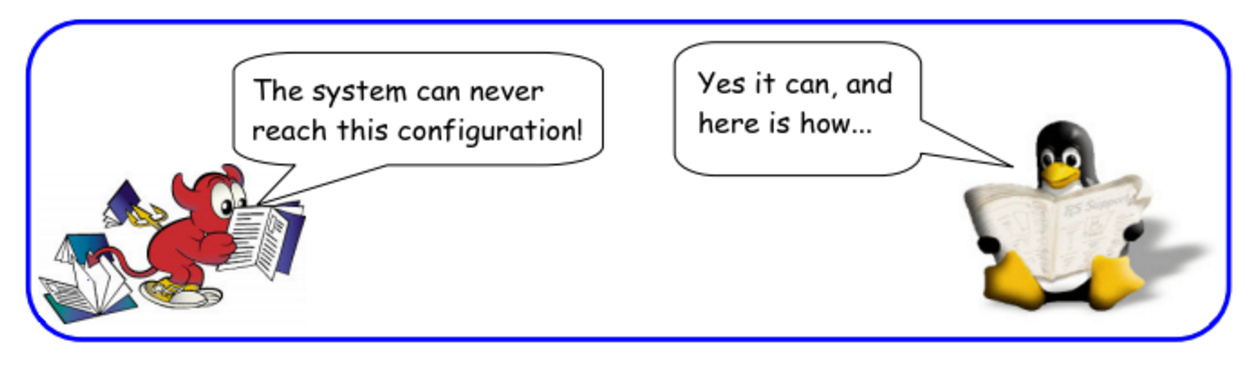
\includegraphics[scale=0.5]{modelchecker}
\caption{Inside Model Checker \cite[]{modelchecker_picture}}
\end{figure}


The model checker allowed us to relax Schelling's turn function, being able to test the systems when agents move in all possible orders. And adding the \textit{fairness} constraints ensured that each agent is picked infinitely often. This is something that cannot be achieved in an object oriented design. Furthermore, we were able to check all the results we got in the \textit{Formal Analysis} Chapter. The series of simulation results we carried out confirmed our formal results in terms of convergence and total segregation of the systems for different turn functions. 

On the negative side, the model (\verb|.smv file|) grows exponentially with each agent added to the system and so does the \textit{Binary Decision Diagram (BDD)} generated by the model checker. This is also known as \textit{The State Explosion Problem} \cite[]{StateExplosionProblem} and it is due, in our model, to a large number of orders in which we allow the unhappy agents to move. To give an example, the \verb|.smv file| that describes the model for 50 agents has over 14 thousand line and when it comes to BDDs, we are talking about millions of possible states. Having so many states for the model checker to cover, means that the execution time for checking a specification can take tens of minutes. However, there are possible solutions to this problem. One of them could be using a \textit{Bounded Model Checking}. This technique is basically checking just a fraction of the entire model. For example, if we want to check that there exists a path to a final configuration that is stable, it is sufficient to find a path in the bounded model and we would be able to say that the property holds in the system as a whole.\\

To summarise, here is a brief list of pros and cons for using a model checker for our multi-agent computational model.

\textbf{Pros:}
\begin{itemize}
    \item Can evaluate whether a variety of proprieties are true of the system model;
    \item It provides counter-examples for properties that do not hold in our system;
    \item It allowed us to use a relaxed version of Schelling's turn function. Hence, we were able to test the impact of turn function in terms of convergence of the system and the level of segregation.
\end{itemize}

\textbf{Cons:}
\begin{itemize}
    \item Challenging to write the system description in \verb|SMV|;
    \item The model grows exponentially with each agent added (State Explosion Problem). Thus, we could run into space and time efficiency problems. However, there are techniques that we could use to avoid these problems, such as \textit{Bounded Model Checking}.
\end{itemize}

\end{document}